\chapter{Fundamentação Teória}
\label{chap:concep}
O termo robô vem da palavra tcheca robota que tem como uma das possíveis traduções “trabalhador forçado” e ganhou o significado atual após o escritor tcheco Karel Capek (1809 - 1938), na sua obra de ficção científica “R.U.R. Rossumovi Univerzální Roboti”, associar o termo às máquinas criadas pelo personagem principal para servi-lo. Mas a ideia de algo que desenvolva atividades de maneira autônoma é apresentada ao mundo muito tempo antes. Aristóteles em \cite{aristoteles1985traduccao} diz: “Se cada instrumento pudesse realizar sozinho a sua tarefa, obedecendo ou antecipando a nossa vontade, [...] os feitores não precisariam de servos, nem os senhores de escravos.” 

Diversas obras da ficção retratam diferentes tipos de robôs criados de forma a reproduzir comportamentos semelhantes aos de um ser humano. Com o passar do tempo, juntamente com o avanço tecnológico nas áreas da eletrônica, mecânica e informática, a construção dessas máquinas se tornou possível. A indústria observou nos robôs, o potencial para automatizar e otimizar as linhas de processo, onde atividades que pudessem demandar mais tempo se fossem executadas por seres humanos, seriam executadas de forma muito mais rápida e precisa com a utilização de máquinas programadas e autônomas, aumentando a produção.

A \cite{iso2012} define um robô como “mecanismo programável atuado em dois ou mais eixos com um grau de autonomia, movendo-se dentro do seu ambiente, para executar tarefas pretendidas”. É resultado da integração de componentes como: Sensores; atuadores; unidade de controle; unidade de potência e manipulador mecânico. Sensores são os componentes que fornecem parâmetros sobre o ambiente em que o robô se encontra e sobre o comportamento do próprio sistema robótico. Já os atuadores são os dispositivos que movimentam as partes, quando convertem energia elétrica, hidráulica ou pneumática em mecânica. A energia necessária para o funcionamento dos atuadores é fornecida pela unidade de potência.

O gerenciamento dos parâmetros necessários para que o robô realize suas tarefas é de responsabilidade da unidade de controle. De onde também são emitidos os comandos para a movimentação. O manipulador mecânico é o conjunto de componentes estruturais do robô, elos ou links, conectados entre si por articulações comumente denominadas de juntas. Graus de liberdade, segundo \cite{romanorobotica} “É o número mínimo de variáveis independentes de posição que precisam ser especificadas para se definir inequivocamente a localização de todas as partes de um mecanismo”.
\begin{flushright}
  Nada é tão maravilhoso que não possa existir, \\
  se admitido pelas leis da Natureza. \\
  \ \\
  (Michael Faraday)
\end{flushright}

\section{Cinemática}\label{sec:cinem}
A cinemática é o ramo da física que descreve o movimento de um corpo, determinando características como posição, velocidade e aceleração. Na robótica, o estudo cinemático resulta em um conjunto de equações que caracterizam o movimento do robô, a complexidade da solução varia com a quantidade de graus de liberdade que esse robô tem. Em um manipulador mecânico composto por links que são conectados por juntas, cada conjunto link-junta caracteriza um grau de liberdade. Dessa maneira, um robô com $n$ conjuntos link-junta tem $n$ graus de liberdade, sendo o primeiro link a base de sustentação do robô no mundo e o último, onde está a seu end-effector.

\subsection{Cinemática Direta}\label{sec:cinem_dir}
A cinemática direta é a solução para a movimentação de um robô com cálculo da posição e orientação do end-effector a partir de dadas posições das juntas. A notação de Denavit-Hartenberg é uma ferramenta utilizada para coordenar a descrição cinemática de sistemas mecânicos articulados com $n$ graus de liberdade.

\begin{figure}[h!]												
	\centering												
	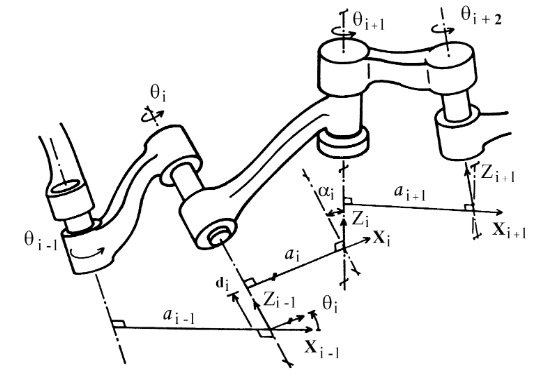
\includegraphics[width=0.5\textwidth]{denavit.png}			
	\caption{Parâmetros de Denavit-Hartenberg}		
	\label{img:denavit}	
	\source{\cite{romanorobotica}}		
\end{figure}

A figura mostra dois \textit{links} ligados por uma junta de superfícies deslizantes uma sobre a outra. Um eixo de uma junta estabelece a conexão de dois \textit{links}. Segundo \cite{romanorobotica}, os eixos das juntas devem ter duas normais conectadas a eles, uma para cada um dos \textit{links}. Assim a posição relativa destes dois \textit{links} conectados ($i-1$ e $i$) é dada por $d_{i}$, que é a distância medida ao longo do eixo da junta entre suas normais. O ângulo de junta $\theta_{i}$ entre as normais é medido em um plano normal ao eixo da junta. Dessa forma, $d_{i}$ e $\theta_{i}$ são a distância e o ângulo entre os \textit{links} adjacentes. Determinam a posição relativa de \textit{links} vizinhos.

Um \textit{link} pode apenas ser conectado a dois outros \textit{links} ($i-1$ e $i+1$). Assim, dois eixos de juntas são estabelecidos em ambos terminais de conexão. Os \textit{links} mantém uma configuração fixa entre as juntas e podem ser caracterizados pelos parâmetros $a_{i}$ e $\alpha_{i}$. O parâmetro $a_{i}$ é a menor distância medida ao longo da normal comum entre os eixos da junta, chamado de comprimento de \textit{twist}, já o $\alpha_{i}$ é o ângulo de \textit{twist}. Esses quatro parâmetros determinam a estrutura do \textit{link}, parâmetros da junta e a posição relativa aos \textit{links} vizinhos.

A representação de Denavit-Hartenberg tem como resultado uma matriz 4 x 4 representando cada sistema de coordenadas do \textit{link} na junta em relação ao \textit{link} anterior. Essa matriz é obtida através do produto das transformações: Translação de uma distância $d_{i}$ ao longo do eixo $Z_{i-1}$ para trazer os eixos $X_{i-1}$ e $X_{i}$ na coincidência; Rotação no eixo $Z_{i-1}$ de um ângulo $\theta_{i}$ para alinhar os eixos $X_{i-1}$ e $X_{i}$; Translação ao longo do eixo $X_{i}$ de uma distância $a_{i}$ para trazer as duas origens na coincidência; Rotação do eixo $X_{i}$ um ângulo $\alpha_{i}$ para trazer os dois sistemas de coordenadas na coincidência. Isso resulta na matriz de transformação homogênea $^{i-1}A_{i}$.

\begin{equation}
^{i-1}A_{i}=T_{z,d} T_{z,\theta} T_{x,a} T_{z,\alpha}=\begin{bmatrix}
1 & 0 & 0 & 0\\ 
0 & 1 & 0 & 0\\ 
0 & 0 & 1 & d_{i}\\ 
0 & 0 & 0 & 1
\end{bmatrix}\begin{bmatrix}
cos\theta_{i} & -sin\theta_{i} & 0 & 0\\ 
sin\theta_{i} & cos\theta_{i} & 0 & 0\\ 
0 & 0 & 1 & 0\\ 
0 & 0 & 0 & 1
\end{bmatrix}\begin{bmatrix}
1 & 0 & 0 & a_{i}\\ 
0 & 1 & 0 & 0\\ 
0 & 0 & 1 & 0\\ 
0 & 0 & 0 & 1
\end{bmatrix}\begin{bmatrix}
1 & 0 & 0 & 0\\ 
0 & cos\alpha_{i} & -sin\alpha_{i} & 0\\ 
0 & sin\alpha_{i} & cos\alpha_{i} & 0\\ 
0 & 0 & 0 & 1
\end{bmatrix}=\begin{bmatrix}
cos\theta_{i} & -cos\alpha_{i}sin\alpha_{i} & sen\alpha_{i}sin\theta_{i} & a_{i}cos\theta_{i}\\ 
sin\theta_{i} & cos\alpha_{i}cos\theta_{i} & -sin\alpha_{i}cos\theta_{i} & a_{i}sin\theta_{i}\\ 
0 & sin\alpha_{i} & cos\alpha_{i} & d_{i}\\ 
0 & 0 & 0 & 1
\end{bmatrix}
\end{equation}

\subsection{Cinemática Inversa}\label{sec:cinem_inv}
Segundo \cite{fu1987robotics} os robôs estão em um espaço onde o objeto a ser manipulado tem sua posição expressa no sistema de coordenadas do ambiente. Com o objetivo de controlar a posição e orientação do \textit{end-effector} do robô, a solução da cinemática inversa é mais adequada. A cinemática inversa consiste em, partindo de uma posição e orientação desejada, calcula-se as posições das juntas para que o robô alcance esse objetivo, é o processo inverso da cinemática direta. 
Há de se observar que a cinemática inversa pode ou não ter solução, caso a posição de interesse esteja fora do espaço de trabalho do robô, não há posições de juntas que execute a tarefa. Nos momentos em que a posição desejada pode ser alcançada, podem existir mais de uma solução. Um ponto importante na solução da cinemática inversa é, quando há mais de uma solução deve-se atentar para qual delas é a melhor opção, levando em consideração o ambiente em que o robô se encontra, principalmente os obstáculos à sua volta. A demanda energética para a execução dos possíveis movimentos e o esforço qual as juntas serão submetidas nesta ação, é crucial para o planejamento da movimentação do robô.


\section{Modelagem Cinemática de um Braço Planar}\label{sec:brac_plan}
O robô ELIR tem na sua estrutura, braços que se movimentam apenas em dois eixos, $x$ e $z$, através da atuação de duas juntas, podendo assim ser modelado cinematicamente como um braço planar do tipo RR. A figura a seguir mostra um exemplo desse braço, RR por ter duas juntas rotativas, que se movimenta no plano $x-y$:

\begin{figure}[h!]												
	\centering												
	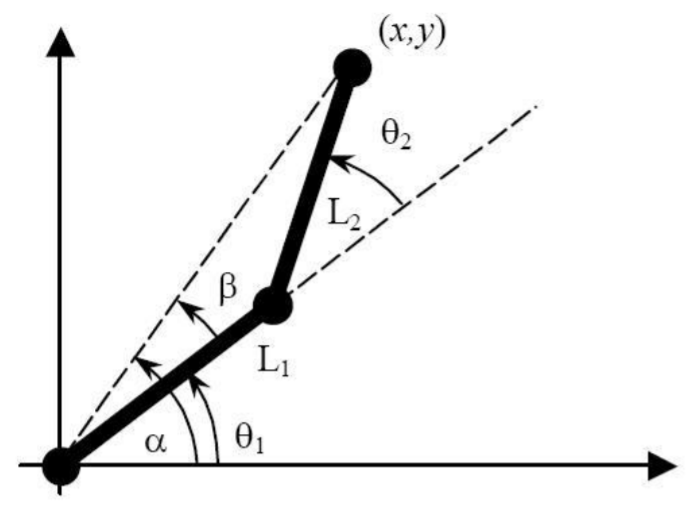
\includegraphics[width=0.5\textwidth]{planar_rr.png}			
	\caption{Braço planar do tipo RR}		
	\label{img:planar}	
	\source{\cite{cinem_inv}}		
\end{figure}

Usando a análise da cinemática direta, consegue-se determinar a posição do \textit{end-effector} com base nos ângulos $\theta_{1}$ e $\theta_{2}$ e nas dimensões $L_{1}$ e $L_{2}$. Logo tem-se que:
\begin{equation}
x=L_1cos{(\theta_1)}+L_2cos{(\theta_1 + \theta_2)}
\end{equation}
\begin{equation}
y=L_{1}sen{(\theta_1)}+L_{2}sen{(\theta_1 + \theta_2)}
\end{equation}
Aplicando a lei dos cossenos ao triângulo formado pelo braço e pela linha entre a origem do braço e o seu \textit{end-effector} obtém-se: 
\begin{equation}
\theta_2=\pm arccos{\frac{(x^2+y^2-(L_1)^2-(L_2)^2)}{2L_1L_2}}
\end{equation}
Para determinar o $\theta_{1}$ considera-se a relação trigonométrica:
\begin{equation}
tan{(A - B)}=\frac{tan(A)-tan(B)}{1+tan(A) tan(B)}
\end{equation}
e tomando:
\begin{equation}
tan(\beta)=\frac{L_2 sin\theta_2}{L_1 + L_2 cos\theta_2}
\end{equation}
tem-se que:
\begin{equation}
\theta_1 = arctan[\frac{y(L_1 + L_2 cos\theta_2)-xL_2 sin\theta_2}{x(L_1 + L_2 cos\theta_2)-yL_2 sin\theta_2}]
\end{equation}
Assim é possível fazer a solução da cinemática inversa para um braço planar RR.

\section{Desenvolvimento de Robôs}\label{sec:desen_robo}
Para o desenvolvimento de sistemas robóticos, é necessária a integração de vários dispositivos, assim sendo necessário utilizar ferramentas e tecnologias que poupem tempo no desenvolvimento, de forma a facilitar o processo de comunicação entre as diversas camadas de abstração. 
As camadas de abstração se referenciam ao alto e baixo nível da máquina, onde baixo nível é uma referência para aplicações mais simples, que estão mais próximas da linguagem da máquina, como por exemplo aplicação de comunicação somente via \textit{bytes}. Um exemplo de um elemento que está numa camada de abstração de alto nível é uma Interface Homem-Máquina , onde o usuário consegue interagir com a máquina diretamente, sem ter que necessariamente entender o seu funcionamento interno.

\subsection{\textit{Framework}}\label{sec:framework}
Em ambientes computacionais, a utilização de ferramentas para realização de atividades e desenvolvimento de soluções é de extrema importância. Estas ferramentas podem ser softwares específicos para execução de uma determinada atividade ou \textit{frameworks}.	
Segundo \cite{tese_framework} “\textit{Frameworks} são estruturas de classes que constituem implementações incompletas que, estendidas, permitem produzir diferentes artefatos de software”. Os \textit{frameworks} em geral permitem o desenvolvimento de soluções computacionais baseadas em determinadas funcionalidades, seguindo uma estrutura definida pelo \textit{framework}. De acordo com \cite{maxwel_framework} os \textit{frameworks} definem uma arquitetura para um conjunto de subsistemas, dando os construtores necessários para a sua criação.
A principal característica de um \textit{framework} é a sua capacidade de reutilização, afinal a sua utilização permite que diversos conjuntos de produtos possam ser gerados partindo de uma única estrutura que possua os conceitos mais gerais.
Segundo \cite{maxwel_framework} \textit{frameworks} podem ser classificados em dois tipos principais: \textit{Frameworks} de Aplicações Orientado a Objetos e \textit{Frameworks} de Componente.
Os \textit{frameworks} orientados a objetos geram famílias de aplicações orientadas a objetos e seus pontos de extensão são definidos como classes abstratas ou interfaces, onde se estendem por cada instância da família de aplicações.
Para \textit{frameworks} de componentes, o suporte é previsto para componentes que sigam um determinado modelo, possibilitando que as instâncias destes componentes sejam acopladas ao \textit{framework}. Também são estabelecidas as condições necessárias para que um componente seja executado, regulando a sua interação entre as instâncias de outros componentes.
Os \textit{frameworks} utilizados para robótica, são extremamente importantes, pois o uso de suas ferramentas possibilita o desenvolvimento e criação das soluções computacionais e códigos necessários para cada funcionalidade de um robô, de forma que o funcionamento delas em conjunto seja otimizado pela natureza do \textit{framework} de realizar a compatibilização entre as estruturas.

\subsection{Simulação}\label{sec:simula}
Em sistemas complexos, onde diversas variáveis definem o seu funcionamento, e por consequência as suas respostas a determinados estímulos, torna-se extremamente difícil e irresponsável executar a sua fabricação antes de realizar uma validação prévia de seu funcionamento.
Este tipo de procedimento de análise prévia do comportamento de um sistema é chamado de simulação. De acordo com \cite{definição_de_simulação} “Simulação refere-se a uma ampla coleção de métodos e aplicações para imitar o comportamento do sistema real, por meio de um computador com um \textit{software} apropriado”. Diversos tipos de sistemas se utilizam da ferramenta de simulação para validar previamente o funcionamento de projetos.
O processo de utilização de uma simulação consiste em basicamente recriar o sistema em questão em um ambiente computacional e então são fornecidas as entradas para o sistema, as rotinas de tratamento destas entradas e por fim as saídas da simulação.

\begin{figure}[h!]												
	\centering												
	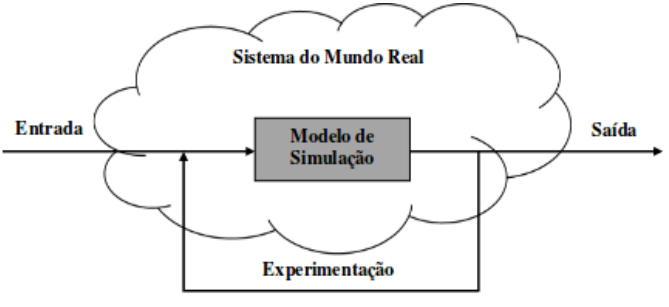
\includegraphics[width=0.5\textwidth]{simulation.png}			
	\caption{Diagrama de funcionamento de um processo de simulação}		
	\label{img:simulation}	
	\source{\cite{definição_de_simulação}}		
\end{figure}


Em sistemas robóticos, uma ferramenta extremamente útil e bastante utilizada, é a simulação. Segundo \cite{artigo_sobre_simulação} 
>“Quando se trabalha com robótica, o uso de uma simulação é de importância significante. Por um lado, ela permite a validação de diferentes alternativas durante o design do sistema robótico, levando assim, a melhores decisões e preservação de custos. Por outro lado, auxilia o processo de desenvolvimento de \textit{software}, disponibilizando uma reposição para robôs que não estejam em mãos”.
Através do uso de \textit{softwares} de simulação é possível criar uma representação computacional não só o modelo físico de um robô, mas também os parâmetros referentes à objetos do ambiente no qual o mesmo será posto em funcionamento. A avaliação prévia da execução das tarefas e do funcionamento do robô, permite a observação do comportamento do sistema em determinadas situações, facilitando assim, a tomada de decisões mais efetivas no processo de desenvolvimento do protótipo real. 

\subsection{Odometria}\label{sec:odom}
A odometria consiste no cálculo para estimar a mudança de posição do robô no tempo, onde isso pode se dar por meio de diversos dispositivos que possibilitem o cálculo de deslocamento. Onde segundo \cite{ben2018robotic}, "Odometria - a medição da distância - é um método fundamental usado por robôs para navegação". A medição de tempo é fácil utilizando o \textit{clock} interno do computador embutido. Medir velocidade é mais difícil: em alguns robôs educacionais utilizam codificadores são usados para contar as rotações da rodas, enquanto em outros a velocidade é estimada das propriedades dos motores. 
No caso da análise de deslocamento do robô na linha por meio de roldanas, o movimento é caracterizado como linear, já que o deslocamento ocorre em somente uma direção, analogamente a odometria utilizada é a linear, onde o deslocamento pode ser calculado simplesmente pela equação \ref{eq:deslocamento} onde $s$ representa o espaço caminhando, $v$ a velocidade e $t$ o tempo. 

\begin{equation}\label{eq:deslocamento}
s = v*t
\end{equation}

Utilizando o medidor de tempo interno do computador embutido nos sistemas robóticos, pode se calcular a variação de espaço para um tempo muito pequeno, onde esses pequenos incrementos são somados ou subtraídos para encontrar o deslocamento do robô.
A velocidade de deslocamento das roldanas pode ser encontrada utilizando a equação \ref{eq:vel} com as informações do raio da roldana $r$ e a sua velocidade de giro $w$ em radianos por segundo. A informação da velocidade de giro da roldana geralmente é extraída dos servomotores utilizados para tração.

\begin{equation}\label{eq:vel}
v = 2\pi*r*w
\end{equation}

O cálculo da odometria por meio da velocidade das rodas é denominado no âmbito da robótica como odometria de roda, \textit{wheel odometry} em inglês, porém, outras técnicas são utilizadas, já que existem diversos tipos de deslocamento diferentes. Outro tipo aplicação muito encontrada é a odometria visual, que segundo \cite{nister2004visual} "Odometria Visual (OV) é o processo de estimação do deslocamento de um agente (ex: veículo, humano e robô) utilizando a entrada de uma ou múltiplas câmeras conectadas a ele". Os domínios da aplicação incluem robótica, realidade aumentada, automotiva e 'computadores vestíveis'.

\subsection{Gestão de Energia}\label{sec:gestao}
O conceito de gestão de energia se dá pela forma como a energia elétrica é utilizada em um sistema composto de diversos dispositivos elétricos e eletrônicos. Para sistemas robóticos, este conceito representa um fator importante para garantir uma operação autônoma de qualidade. Os robôs quando nesse tipo de operação, geralmente não dispõem de uma fonte de energia constante, e portanto, são geralmente alimentados por baterias e tendo interação por meio de conexões sem fio. 
O uso de diversos dispositivos eletrônicos de baixo consumo energético, como sensores e interfaces microcontroladas, podem não se mostrar um problema para um curto período de operação, porém, para maximizar o tempo da atividade exercida pelo robô, é necessário encontrar uma forma eficiente de gerir a operação dos dispositivos conectados na rede de alimentação. Segundo \cite{katiraei2006power} 
>“Gestão de energia é um conceito importante em redes de sensores, porque uma estrutura de energia cabeada geralmente não está disponível e um conceito óbvio é utilizar a energia disponível da bateria de forma eficiente”. 	
Quanto mais atividades diferentes o robô desempenha maior será a demanda de energia entre os dispositivos interconectados, isso faz com que seja necessário que os desenvolvedores busquem uma forma de otimizar o custo de energia individual das atividades e do fluxo de operação como um todo. Os diversos dispositivos utilizados em sistemas robóticos fazem com que o mesmo se utilize de diferentes níveis de tensão e corrente, já que comumente, os dispositivos utilizados são comerciais, e devido às diferenças das suas características e parâmetros, definidos por empresas diferentes, responsáveis pela produção e fabricação das ferramentas, é necessário que a gestão de energia leve em consideração a compatibilidade entre diferentes dispositivos.

\subsection{Conceito de segurança e Integridade}\label{sec:segur_inte}
Em diversas áreas, é comum a verificação das condições antes da execução de atividades, a aviação é um grande exemplo de uso desse conceito. Neste seguimento, o \textit{checklist} é utilizado toda vez antes de um avião decolar, assim é possível verificar se os sistemas vitais para o vôo estão em ordem. O principal objetivo dessa ação é identificar os riscos que existem para o cumprimento da atividade.
Para que um dispositivo robótico execute as tarefas para as quais ele foi desenvolvido, deve-se verificar se os seus sistemas, como um todo, e os componentes individualmente, estão em condições de funcionamento, garantindo assim a integridade do sistema como um todo. Essa análise deve ser feita levando em conta a importância de cada sistema e de cada componente desses sistemas, a fim de aumentar a capacidade de operação em condições adversas do robô. Podem existir sistemas que, mesmo quando não estão operando adequadamente, não comprometem a execução da missão do robô.

\subsection{Comunicação em sistemas robóticos}\label{sec:comm_sis}
Dispositivos eletrônicos são capazes de realizar transmissão de dados, afinal, a interconexão entre eles é de extrema importância em sistemas em que existam diversos dispositivos responsáveis por funções distintas. Dispositivos que se comunicam entre si, são capazes de criar uma rede em todo o sistema, permitindo um aumento na confiabilidade das funções do sistema, através da troca de informações de parâmetros que venham a ser importantes para o funcionamento do sistema como um todo.
Para que os dispositivos possam se comunicar entre si, os mesmos adotam o que se chama de protocolos de comunicação. Protocolos de comunicação são arquiteturas que estabelecem a troca de dados entre dispositivos eletrônicos. Os dispositivos comerciais possuem diferentes tipos de protocolos de comunicação e por isso, torna-se extremamente importante se atentar a qual protocolo utilizar durante a conceituação de um projeto que se tenha a necessidade da interconexão de dispositivos.
Uma das formas mais comuns de se realizar a transmissão de dados entre dispositivos embarcados é a comunicação serial. \cite{livro_sistemas_embarcados} define a comunicação serial como um envio de \textit{bits} de forma serial, similar a uma fila. Possuindo dois canais principais: o canal $TX$ para envio e o canal $RX$ para recebimento. Dentro desse processo de comunicação alguns parâmetros devem ser levados em conta, como a taxa de transmissão de dados (\textit{BaudRate}); bits de paridade, para assegurar que o número de bits no campo de dados é par ou ímpar; bits de parada para indicar o início ou fim de uma comunicação.
Outro meio de comunicação muito utilizado é o USB (\textit{Universal Serial Bus}), criado com a intenção de tornar a comunicação serial mais simplificada e com uma taxa de transmissão muito mais elevada. Os cabos conectores USB possuem geralmente quatro fios condutores, sendo dois deles para alimentação e dois outros cabos de dados. Os cabos de dados são nomeados como D+ e D-, onde a comunicação entre os dispositivos se dá pela variação de tensão entre estes dois sinais.
Dentro de ampla complexidade como um robô, onde diversos dispositivos necessitam estar trocando informações, a utilização de protocolos de comunicação serial se tornam extremamente importantes para a garantia da confiabilidade na execução de tarefas e operações.
